\documentclass[acmtog, anonymous,review, nonacm, balance = false]{acmart}
%%
%% \BibTeX command to typeset BibTeX logo in the docs
\AtBeginDocument{%
  \providecommand\BibTeX{{%
    \normalfont B\kern-0.5em{\scshape i\kern-0.25em b}\kern-0.8em\TeX}}}

\usepackage{xcolor}
\usepackage{colortbl}
\usepackage{bbm}
\usepackage{algorithm}
\usepackage{algpseudocode}
\usepackage{wrapfig}

%font stuff
\DeclareMathAlphabet{\mathpzc}{OT1}{pzc}{m}{it}
\newcommand{\reftbl}[1]{Table~\ref{tbl:#1}}
\newcommand{\reffig}[1] {Fig.~\ref{fig:#1}}
\newcommand{\refalg}[1] {Alg.~\ref{alg:#1}}
\newcommand{\refeq}[1] {Eq.~\ref{eq:#1}}
\newcommand{\refsec}[1] {\S\ref{sec:#1}}

%notes on
%\newcommand{\dave}[1]{{\bf\textcolor[rgb]{0.2,0.2,0.8}{Dave: #1}}}
%\newcommand{\ty}[1]{{\bf\textcolor[rgb]{0.8,0.2,0.2}{Ty: #1}}}
%\newcommand{\Honglin}[1]{{\bf\textcolor[rgb]{0.2,0.8,0.2}{Honglin: #1}}}
%\newcommand{\nicetohave}[1]{{\bf\textcolor[rgb]{1,0,0}{Nice To Have: #1}}}
%\newcommand{\revise}[1]{{\textcolor[rgb]{0.9,0.4,0.14}{#1}}}

%notes off
\newcommand{\dave}[1]{}
\newcommand{\ty}[1]{}
\newcommand{\Honglin}[1]{}
\newcommand{\nicetohave}[1]{}
\newcommand{\revise}[1]{}

%%% Math Symbols below %%%%
\newcommand{\real}{{\rm I\!R}}
\newcommand{\integer}{\mathbb{Z}}
\newcommand{\vc}[1]{\mathbf{#1}}
\newcommand{\refX}{\mathbf{X}}
\newcommand{\defX}{\mathbf{x}}
\newcommand{\Jnurbs}{J}
\newcommand{\ident}{I}
\newcommand{\Pmat}{P}
\newcommand{\Pco}{\vc{c}}
\newcommand{\tr}{\vc{t}}
%\newcommand{\Pmatx}  {\begin{bmatrix}\Pmat\left(\refX\right) & \ident \end{bmatrix}}
%\newcommand{\Pmatxuv} {\begin{bmatrix}\Pmat\left(\refX\left(u,v\right)\right) & \ident \end{bmatrix}}
\newcommand{\Pmatx}{\Pmat\left(\refX\right)}
\newcommand{\Pmatxuv}{\Pmat\left(\refX\left(u,v\right)\right)}
\newcommand{\Pmatxi}{\Pmat_i\left(\refX \right)}

\newcommand{\Pcox} {\begin{bmatrix} \Pco\\ \tr \end{bmatrix}}
\newcommand{\samp}[1]{\hat{#1}}
\newcommand{\wt}{S}
\newcommand{\ar}{a}
\newcommand{\vol}{v}
\newcommand{\bld}{w}
\newcommand{\bldxi}{\bld_i\left(\refX\right)}
\newcommand{\bldmat}{W}
\newcommand{\prt}{\mathpzc{b}}
\newcommand{\Prts}{\mathpzc{B}}
\newcommand{\XBs}{\bar{\mathpzc{X}}}
\newcommand{\st}[1]{\mathpzc{#1}}
\newcommand{\clst}{\refX^*}
\newcommand{\rhit}{\refX^h}
\newcommand{\orgn}{\bar{\refX}}
\newcommand{\MM}{M}
\newcommand{\ME}{M_\epsilon}
\newcommand{\fo}{\vc{f}}
\newcommand{\fext}{\vc{f_{ext}}}
\newcommand{\shapef}{N}
\newcommand{\Jkin}{\Gamma}
\newcommand{\defo}{F}
\DeclareMathOperator{\Tr}{Tr}
\DeclareMathOperator*{\argmin}{arg\,min}



\acmSubmissionID{230}
\newcommand\myworries[1]{\textcolor{red}{#1}}

%%%%%%%%%%%%%%%%%%%%%%%%%%%%%%%%%%%%%%%%
% Inverting Colors to save my eye balls
%\usepackage{xcolor}
%\pagecolor[rgb]{0.1,0.12,0.15}
%\color[rgb]{.9,.9,.95}
%%%%%%%%%%%%%%%%%%%%%%%%%%%%%%%%%%%%%%%%

\citestyle{acmauthoryear}

\begin{document}

\title{The Shape Matching Element Method: Direct Animation of Curved Surface Models}

%% A "teaser" image appears between the author and affiliation
%% information and the body of the document, and typically spans the
%% page.
\begin{teaserfigure}
  \includegraphics[width=\textwidth]{figures/teaser_castle.pdf}
  \caption{Using the shape matching element method we can directly simulate this NURBS surface model of a bouncy castle as a volumetric elastic object without the need for volumetric meshing of any kind.}
  \label{fig:teaser}
\end{teaserfigure}

\begin{abstract}
We introduce a new method for direct physics-based animation of volumetric curved models, represented using NURBS surfaces.  
Our technical contribution is the Shape Matching Element Method (SEM).
SEM is a completely meshless algorithm, the first to simultaneously 
be robust to gaps and overlaps in geometry, 
be compatible with standard constitutive models and time integration schemes, support contact and frictional interactions  
and to preserve feature correspondence during simulation which enables editable simulated output. 
We demonstrate the efficacy of our algorithm by producing compelling physics-based animations from a variety of curved input models.
\end{abstract}

\maketitle

\section{Introduction}

The consumption of geometric surface models by physics-based animation algorithms is fraught with difficulty. 
For volumetric objects, this process often involves identifying and discretizing the interior of the modelled object, 
typically either as a tetrahedral or hexahedral mesh.%
This procedure is both expensive and difficult, especially if the surface model is constructed from higher-order boundary
representations, or if the volumetric discretization is required to be conforming or feature aligned. 
Removing explicit volumetric discretization from the physics-based-animation pipeline can avoid these difficulties and 
also provide a more unified modelling and simulation experience. 

NURBS (Non-uniform Rational B Splines) are a popular higher-order modelling primitive which 
are used for computer-aided design (CAD), computational fabrication and computer animation. 
NURBS primitives were the first geometric representation used for physics-based animation, yet,
despite over three decades of research, animation of NURBS objects remains a challenge.

Isogeometric Analysis (IGA) is a physics simulation methodology that uses the control variables of the NURBS model
as the degrees-of-freedom (DOFS) of the simulation itself. 
Unfortunately IGA approaches for volumetric objects still require background volumetric structures, typically
regular grids that make satisfaction of boundary conditions difficult (which makes collision resolution difficult)
or more complicated cut-cell grids which introduce non-trivial root finding problems into the mix. 
Crucially, these simulation schemes typically assume models arise from engineering applications and meet tight geometric
criteria such as that the mesh is manufacturable. 
These inputs are much cleaner than those produced by a typical modeller. 

% In this paper we present a new finite element method for isogeometric, physics-based animation of NURBs models.
% Crucially our method is boundary only, and requires no volumetric meshes (thus avoiding their inherent complications), grids or cutcells of any kind
% Our method does not need an explicit labelling of the inside/outide of the simulated model
% Does not require nurbs patches in an object to be explicitly joined
% Input is just the raw NURBs model with no additional information or annotations
% The resulting simulation algorithm is compatiable with nonlinear continuum mechanics material models as well as 
% standard methods for contact resolution. 

We present the first truly meshless (no volumetric discretization generated) algorithm for direct, nonlinear elastodynamic simulation of NURBs models. 
Our nonlinear elastodynamic simulation scheme requires only a boundary description of the object (we do not strictly require a solid model) and
approriate physical parameters.  
Because we explicitly use the NURBS boundary representation in the simulation its is straightforward to handle
Dirichilet, Neumann boundary conditions and to apply contact resolution. 
Crucially because we broadly target animation not necessarily simulation for engineering or manufacturing we don't require that models
satisfy the rigourous geometric requirements common for these applications

Our approach is an extension of the recently developed Virtual Element Method (VEM) for solving PDEs on domains tiled with arbitrary polygons.
We establish a connection between VEM and the well-known shape matching simulation algorithm  which enables us 
to derive equations of motion for an arbitrary NURBS model using Lagrangian Mechanics. 
Importantly, we show how to replace volumetric data structures for integration with ray casting approaches which enables
our meshless approach to isogeometric elastodynamic simulation of volumetric structures.

% Modelling -> Animation -> Rendering
% Use physics for animation which requires conversion from modelling to simulation representation
% for volumetric objects this conversion invovles identififyin and meshing the interior of the modelled object and that's hard
% especially difficult if object surface is described by higher-order boundary representations. 
% Ideally we would have a more direct method of translating our surface model into a volumetric, simulatable form
%
% NURBs  are an oft-used higher order modelling primitive popular for CAD and Computer Graphics for which nice modelling tools exist
% Rhinocerous 3D and Fusion 360.
% Despite lots of work performing physics-based animation on NURBS models is hard
% robustly uilding a volumetric polygonal mesh that simulataneously maintains a corresonpondence to the model surface is an open-research problem
% Isogeometric approaches which directly use the NURBs primitives as simulation variables require additional background grids, complex cutcell algorithms
% and often must rely on soft boundary conditions.
%
% Want to say there is an advantage to avoiding constructing volumetric representations because it costs time and adds complexity
% that;s our goal to provide an alternative, the first truly meshless approach to IGA which maintains a tightt mapping to the boundary
% In this paper we present a new finite element method for isogeometric, physics-based animation of NURBs models.
% Crucially our method is boundary only, and requires no volumetric meshes (thus avoiding their inherent complications), grids or cutcells of any kind
% Our method does not need an explicit labelling of the inside/outide of the simulated model
% Does not require nurbs patches in an object to be explicitly joined
% Input is just the raw NURBs model with no additional information or annotations
% The resulting simulation algorithm is compatiable with nonlinear continuum mechanics material models as well as 
% standard methods for contact resolution. 
%
% crucially because we broadly target animation not necessarily simulation for engineering or manufacturing we don't require that models
% satisfy rigourous geometric requirements common for these applications
%
% Our approach relies on the recently developed Virtual Element Method for solving PDEs on domains tiled with arbitrary polygons.
% By establsihing the connection between VEM and the well-known shape matching simulation algorithm we derive equations of motion sfor 
% an arbitrary NURBS model using Lagrangian Mechanics. We avoid using volumetric data structures for integration by demonstrating that 
% raycasting provides a fast and reliable alternative. In combination, our contributions amount to the first algorithm for 
% isogeometric elastodynamics of volumetric structures that is truly meshless (introducing no auxilillary volumetric data structures) 
% which serves to close the considerable gap betweeen modelling and physics-based animation. 
%
% Desiderata for a sucessful algorithm for PBA 
% No volumetric mesh creation
% Support for Nonlinear Constitutive Models
% Support for standard Collision 
% DOFS on the Boundary (useful for boundary conditions, contact)
% Automatic determination of model volume
% Non-manufacturable models 
% Code Available 

%limitations
% sometimes you want some volumetric dofs to better resolve internal behaviour
\section{Related Work}

%% Set the scene
Geometric modeling is a necessary precursor to physics-based animation, however connecting differing geometric representations for modelling and simulation often requires
time-consuming, complex geometry processing pipelines. 
For instance, the popular tetrahedral finite element approach for simulating solid elastodynamics~\cite{10.1145/2343483.2343501} requires robust algorithms for converting input surface geometry into 
a volumetric tetrahedral mesh. This is a difficult problem and while significant progress has been made,
even the most robust volumetric methods~\cite{Hu:2018:TMW:3197517.3201353} can be time consuming, fail to maintain correspondence between the input model and output simulation mesh,
and don't work directly on curved surface representations such as NURBS.  

%% Outline desiderata for success
%- no meshing of any kind, no tet, hex cut cells, nothing
%- simulation can be directly imported and edited in modelling software
%- supports standard continuum mechanics constitutive models
%- supports different time integrators (can show a few maybe linearly implicit, fully implicit and RK4 ?)

For many physics-based animation tasks, it would be desirable to bypass volumetric meshing entirely and directly simulate the geometric model.
An ideal approach would avoid meshing of any kind (no volumetric meshes or cut-cells), support continuum mechanics-type constitutive models 
and energies that have become standard in physics-based animation pipelines, be compatible with a wide range of time integration schemes and
ensure that simulation output can be edited in the same modelling software used to create the input (important for post-processing). 
Finally, our method should put only moderate constraints on input model quality to facilitate ease-of-use.

\emph{Isogeometric Analysis}~\cite{10.1002/9780470749081.ch7} endeavors to perform simulation directly on the NURBS output from 
Computer-Aided Design (CAD) software. Initial attempts used NURBS surfaces to represent the medial surface of thin objects~\cite{10.1145/176579.176580}.
Volumetric simulations relied on volumetric NURBS~\cite{10.1007/978-3-642-03596-8_2} but were limited to a narrow class of geometries.
Finite volume methods are applicable to more general geometries~\cite{HEINRICH20121645,10.1002/nme.2311} but require a volumetric mesh to be generated.
Modern approaches are constructed around the extended finite element method which enriches the standard finite element basis with discontinuous basis functions
to improve boundary handling~\cite{https://doi.org/10.1002/nme.3120,10.1007/s00466-013-0854-7,https://doi.org/10.1002/nme.4852,SAFDARI2016373,10.1145/3355089.3356576}. 
These methods typically start with an easy-to-generate structured volumetric mesh (tetrahedral or hexahedral), ``cutting'' the NURBS geometric model against
it to enable boundary handling (such a mesh is called a \emph{cut-cell} mesh). 
Like volumetric meshing, this cutting operation can be difficult and our ideal method would avoid it. 
Some cut-cell algorithms assume engineering/manufacturing quality input, which puts tight requirements on input models~\cite{10.1145/3355089.3356576}.
Finally these approaches require additional mechanisms to ensure that simulation results lie inside the shape space of the input model's primitives,
which increases the complexity. 

\revise{
\emph{Embedded Methods} attempt to sidestep many of these issues by enclosing complex surface geometry inside a simulation coarse mesh~\cite{10.5555/1009379.1009573}. 
However, producing an appropriate mesh embedding introduces a number of challenges since the coarse mesh's connectivity must mirror that of the embedded surface.
This necessitates the use of complex hierarchical methods like that of~\citet{10.1145/1531326.1531358}, which themselves require the user to correctly intuit an appropriate ultimate grid resolution.
Alternately one can introduce cut cell~\cite{Tao:Mandoline:2019} or extended Finite Element~\cite{10.1145/3355089.3356576} approaches which bring with them complicated geometric operations. 
Furthermore when the DOFs do not lie on the boundary, methods such as Nitsche's Method ~\cite{Nitsche1971berEV} are required for handling Dirichlet boundary conditions. 
Our method inherits shape connectivity directly from the boundary input, avoiding these difficulties entirely.
}

\emph{Shape Matching} is a meshless approach to physics-based animation~\cite{10.1145/1073204.1073216,10.1145/2019406.2019438} and geometry processing~\cite{10.1111/j.1467-8659.2012.03171.x}
built around shape registration. The algorithm has been extended from volumetric triangle mesh input to cloth~\cite{10.2312/PE/vriphys/vriphys08/039-046}, to particles~\cite{10.1145/1964921.1964987}
and even to visual geometry for video games~\cite{10.1145/2994258.2994260}. 
Shape Matching is fast~\cite{10.1145/1275808.1276480,10.5555/1632592.1632606} and meshless, but state-of-the-art methods require 
additional modelling input to position simulation primitives~\cite{10.1145/1964921.1964987} or limit simulation primitives to be 
collections of convex polytopes~\cite{10.1145/2994258.2994260}.
Finally, Shape Matching is tightly coupled to the position-based dynamics (PBD)~\cite{muller2007position}
time integration methodology. 
While incredibly performant, this approach is incompatible with the constitutive models that are popular for physics-based animation, as well as 
other time integration schemes. 
The popular Projective Dynamics algorithm~\cite{10.1145/2601097.2601116} enables a more flexible Shape Matching implementation but is still limited to a subset of
constitutive models for elastic solids. 

To alleviate these restrictions we turn to other meshless methods popular in computer graphics and 
engineering~\cite{10.1145/1028523.1028542,https://doi.org/10.1002/fld.1650200824,10.1145/1778765.1778776,10.1145/2010324.1964968, 10.1145/1944846.1944855}.
These methods support more advanced constitutive models and integration schemes but often require background integration meshes, limit themselves to low order deformation functions 
and lose the direct connection with
modelling geometry. 
Like cut-cell-based, Isogeometric Analysis approaches, additional constraints must be added to ensure that simulation output can be represented by the input model.
Given this, we conclude that there is no existing algorithm that meets our desiderata for success. 

Our algorithm takes the Shape Matching approach as inspiration, but rather than follow the PBD formalism, we interpret Shape Matching as a 
Virtual Element Method (VEM)~\cite{10.1142/S0218202512500492,10.1142/S021820251440003X}. Virtual Elements are an extension of 
mimetic finite differences~\cite{10.1142/S0218202505000832,10.1016/j.jcp.2013.07.031} to weak-form variational problems. 
VEM relaxes the mesh generation requirements of the finite element method by enabling the solution of partial differential equations
on domains partitioned with arbitrary polytopes~\cite{10.1145/3386569.3392389}. 
The solution inside each polytope is approximated using a polynomial function of a specified order.
VEM typically assumes that the boundary of the the problem domain is described by a piecewise linear complex
which makes its standard formulation incompatible with our curved input geometry. 


\subsection*{Contributions} 
In this paper we develop a new Shape Matching-based, Virtual Element Method which is directly compatible 
with NURBS input geometry rather than piecewise linear surfaces. 
Furthermore, we improve the expressivity of the VEM basis by using a shape blending approach inspired by
algorithms for skinning~\cite{skinningcourse:2014}.
Our method is entirely meshless (requiring no volumetric meshes or cut-cells) and is compatible with standard constitutive models and time integrators.
It guarantees that simulation output is directly consumable by the input modelling software and can ingest models which include large gaps,
intersections and disconnected primitives without additional user input. 
These features mean that our algorithm is the first truly meshless approach for the direct simulation of curved surface, NURBS models in physics-based animation.

%\subsection{Virtual Element and other Element Methods}
%\begin{enumerate}
    %\item \textit{Mimetic Finite Differences} \cite{10.1142/S0218202505000832} \cite{10.1016/j.jcp.2013.07.031} (they double dipped!): Considered a close relative to VEM and framed as the predecessor to VEM (in VEM papers). I still haven't read on MFD yet. From PolyDDF: "extension of finite volume and finite difference techniques to polygons that first discretizes a prime operator (typically, the gradient or the divergence) via a boundary integral, and then derives other operators by mimicking continuous structural properties."
    %\item \textit{Basic principles of Virtual Element Method} \cite{10.1142/S0218202512500492} Original VEM paper
    %\item \textit{The Hitchhiker's Guide to Virtual Element Method} \cite{10.1142/S021820251440003X}: More understandable versions of original VEM paper.
    %\item \textit{Discrete Differential Operators on Polygonal Meshes} \cite{10.1145/3386569.3392389}: Extends VEM to do discrete differential geometry on arbitrary polygonal meshes.
    %Don't think we need to cite this \item \textit{FLexible Simulation of Deformable Models using Discontinuous Galerkin FEM} \cite{10.5555/1632592.1632608}: Uses ordinary hexahedral elements, but uses a cut cell-based approach to support arbitrary polyhedra on the surface. 
    %Later ?\item \textit{Generalizing the finite element method: Diffuse approximation and diffuse elements} \cite{Nayroles1992GeneralizingTF} Predecessor to Element Free Galerkin. FEM interpolation replaced with a local Moving Least Square interpolation.
    %Later ?\item \textit{Element-free Galerkin methods} \cite{https://doi.org/10.1002/nme.1620370205}: similar to DEM, but more accurate gradients (not sure of all the differences). In MLS methods, they solve least squares for each particle in the domain, weighting nearby particles with a Gaussian-like density function. In contrast to us, we only compute least squares fitting on the boundary, and then precompute some weighting for each particle to the projection operators on the boundaries.
    %\item \textit{Unified Simulation of Elastic Rods, Shells, and Solids} \cite{10.1145/1778765.1778776}: Propose Generalized moving least squares (GMLS) to resolve limitation of MLS shape functions that require many particles in the support of a point (that are not coplonar).  
%\end{enumerate}


%\subsection{Shape Matching Related Papers}
%\begin{enumerate}
%    \item \textit{Shape Matching} \cite{10.1145/1073204.1073216}: Meshless simulation by fitting a polynomial describing the shapes deformation using only the nodal values.
    %\item \textit{Lattice Shape Matching} \cite{10.1145/1275808.1276480}: Voxelize model to construct a lattice of cubes. Use these lattice cubes to construct overlapping shape matching regions (just like clustered shape matching?). The original mesh is deformed using trilinear interpolation of lattice vertex positions.
    %\item \textit{Robust Real-Time Deformation of Incompressible Surface Meshes} \cite{10.1145/2019406.2019438}: Shape matching on trimeshes with overlapping regions (clustered shape matching). Adds an additional volume preservation constraint. Position based dynamics approach to satisfying volume preservation.
 %   \item \textit{Shape-Up: Shaping Discrete Geometry with Projections} \cite{10.1111/j.1467-8659.2012.03171.x}: Shape constraints by least squares fitting (like in shape matching). They have some "proximity function" indicating distance to least-squares fit, then uses projection operators to minimize proximity function (pretty much just shape matching). 
    %\item \textit{Shape Matching with Oriented Particles} \cite{10.1145/1964921.1964987}: More general form for shape matching, permitting wider range of motion. Also they use shape matching projection operators for skinning, much like we do. For each skinning point, they specify weights with up to 4 particles (each with their own projection operator)
    %\item \textit{Fast Adaptive Shape Matching Deformations} \cite{10.5555/1632592.1632606}: Essentially same thing as Lattice Shape Matching, but instead they use an octree instead of a basic voxel grid for shape matching. It's not super significant to mention this paper, but it does make clear that much of the followup work after shape matching never didn't emphasize it's utility as a meshless boundary only method. They kept converting it to a mesh-based method!
    %\item \textit{A Geometric Deformation Model for Stable Cloth Simulation} \cite{10.2312/PE/vriphys/vriphys08/039-046} Shape matching for cloth simulation.
%\end{enumerate}
%% start with iso geometric analysis (XCAD here)
%\subsection{Isogeometric Analysis}
%\begin{enumerate}
    %\item \textit{Isogeometric Analysis Book} \cite{10.1002/9780470749081.ch7}: The book everyone references when they write Isogeometric analysis in their papers.
    %\item \textit{Dynamic NURBS} \cite{10.1145/176579.176580}: Outline of how to simulate on NURBS with the control points as the degrees of freedom. Method used in our work.
    %\item \textit{XCAD} \cite{10.1145/3355089.3356576}: Optimize CAD models. CAD embedded in hexahedral mesh, complex integration strategy. Uncut hexahedral elements simulated ordinarily, cut elements use XFEM that add additional DOF to account for new element shapes.
    %\item \textit{Development of a quadratic finite element formulation based on the XFEM and NURBS} \cite{https://doi.org/10.1002/nme.3120}: XFEM to handle curve surface integration of NURBs patches. Complex subdividing of "X-Elements" to produce cut cells along NURBS surfaces.
    %\item \textit{A NURBS enhanced extended finite element approach for unfitted CAD analysis} \cite{10.1007/s00466-013-0854-7}: Pretty much the same as the quadratic, but allows higher-order approximation and better handling of interface.
    %\item \textit{A NURBS-based interface-enriched generalized finite element method for problems with complex discontinuous gradient fields} \cite{https://doi.org/10.1002/nme.4852}: Similar to other XFEM NURBS approaches. Uses NURBS-based enrichment functions with cut cells. Additional DOFs added to handle discontinuities.
    %\item \textit{A NURBS-based generalized finite element scheme for 3D simulation of heterogeneous materials} \cite{SAFDARI2016373}: Similar to previous "NIGFEM" paper above, but now in 3D.
    %\item \textit{Swept Volume Parameterization for Isogeometric} \cite{10.1007/978-3-642-03596-8_2} To provide volumetric simulation of NURBS they introduce a new NURBS volume parameterization (B-Spline Volumes ... jesus christ)
    %\item \textit{A finite volume method on NURBS geometries and its application in isogeometric fluid–structure interaction} \cite{HEINRICH20121645}: Combines NURBS paramaterization with finite volume method (requiring a mesh for the volume). 
    %\item \textit{NURBS-Enhanced Finite Element Method (NEFEM)} \cite{10.1002/nme.2311}: Similar to the above example. They run an order FVM simulation and deal with the interface in a complicated manner (could this be considered XFEM?).
%\end{enumerate}


%% start with standard fem stuff
%% start with iso geometric analysis (XCAD here)
%% talk about shape matching and simulating visual geometry but not constitutive models
%% talk about how sparse mesh free methods fixes these things but still loses connection to modelling geometry
%% - ^^^ throw rig space physics in here talk about constraints talk about finding method that does this by construction but is still meshes.
%% talk about VEM has a potential solution 
%% limitation is that it looks at piecewise linear stuff, one polynomial per element, limits expressivity




%\subsection{Other Meshless Methods in Graphics}
%\begin{enumerate}
    %\item \textit{Point Based Animation }\cite{10.1145/1028523.1028542}: Purely particle based, MLS to approximate derivatives. Appears to be among the earliest meshless methods in graphics based on continuum mechanics. 
    %\item \textit{Position Based Dynamics} \cite{MULLER2007109}: Operates directly on particle positions by forming set of constraints and solving for particle positions that satisfy these constraints. Meshless
    %\item \textit{Projective Dynamics} \cite{10.1145/2601097.2601116}: Similar to position based dynamics but solves the constraints implicitly by minimizing energy potentials. Mesh-based. Global solver unlike PBD which satisfies constraints locally using Gauss-Seidel.
%\end{enumerate}

%%% Might need later in methods section
%\subsection{Physics based Skinning}
%\begin{enumerate}
%    \item \textit{Skinning Siggraph Course} \cite{10.1145/2614028.2615427}: The linear weighting of polynomials at the exterior is very similar to skinning.
%    \item \textit{Linear Subspace Design for Real-Time Shape Deformation} \cite{10.1145/2766952}: Linear deformation subspace that uses linear blend skinning and generalized barycentric coordinates. Similarly, we have "handles" but they are represented by entire NURBS patches, and our coordinates are the output of a polynomial, whereas barycentric coordinates are linear (I only skimmed this paper, not sure if this description is fair).
%    \item \textit{Complementary dynamics} \cite{Zhang_2020}: Physics based skinning, orthogonality constraint can be seen as similar to our stability term (conformity term, error term, whatever it's called :))
%    \item \textit{Physically-Based Character Skinning} \cite{10.2312/PE.vriphys.vriphys13.025-034}: Linear blend skinning with multiple layers of skin simulated via oriented particle shape matching and position based dynamics to enforce distance constraints (avoiding unwanted intersections).
%\end{enumerate}

%Might need later in methods
%\subsection{Quadrature}
%\begin{enumerate}
%    \item \textit{A new method for meshless integration in 2D and 3D Galerkin meshfree methods} \cite{KHOSRAVIFARD201030}: Strategy we use for integrating over CAD model volumes. Raycast along single dimension, find intersections, generate quadrature points in the intervals inside the object.
%    \item Adaptive image-based intersection \cite{DBLP:journals/tog/WangFP12}: related to our meshless integration strategy in that we could use this to account for errors in the above approach (increase ray density where we estimate high error to be)
%    \item Efficient and accurate numerical quadrature for immersed boundary methods \cite{10.1186/s40323-015-0031-y}: Finite Cell Method. "Immerses" a shape in a set of cells (mesh!) and computes quadrature over this. To handle curved surface they use an octree to subdivide to the desired level of accuracy.
%    \item Higher-Order Finite Elements for Embedded Simulation \cite{10.1145/3414685.3417853}: Another Finite Cell method like the above, but with a new quadrature generation method (the ones with the circles in the triangles)
%    \item \textit{Highly accurate surface and volume integration on implicit domains by means of moment-fitting} \cite{https://doi.org/10.1002/nme.4569} and \cite{https://doi.org/10.1002/nme.5343}: XCAD paper extends upon this method \myworries{still need to read these}
%\end{enumerate}

%Might need later
%\subsection{Misc}
%\begin{enumerate}
%	\item TRACKS: Toward Directable Thin Shells \cite{10.1145/1276377.1276439}: Petrov-Galerkin test functions for weak-form constraints that handles artifacts due to pointwise constraints.
    %\item Fusion 360 Gallery \cite{willis2020fusion} : source of some models
%\end{enumerate}
%A pointform description of the general idea
%\begin{itemize}
%	\item A D-NURBS approach to simulation. Use a Jacobian to map from UV positions in a NURBS parametric space to world space positions on the surface. 
%	\item \textbf{Shape Matching}: From the sample world space positions on a single NURBS surface, we solve a least squares problem to fit a \textit{projection operator} to the surface. This projection operator maps monomials in the undeformed space, to the least squares estimate of the deformed positions for the given monomials.
%	\item With DNURBS and Shape Matching VEM we have two mappings: a UV to undeformed world space with our NURBS Jacobian, then an undeformed to deformed mapping with the projection operators. This lets us form a set of generalized coordinates in terms of our control points of the NURBS surface (section 1.4).
%	\item For an arbitrary position in space (not necessarily on the surface), we can build a projection operator unique to this point via a weighted sum of the projection operators of the projection operators for each NURBS (eq 5). From this we can reconstruct an estimate of the deformed position from the monomial basis defined using its undeformed position.
%	\item For any point in space, we need to compute a set of weights to the projection operators defined on the surfaces with the following criteria: the weights sum to 1, are nonzero, and depend on the distances to the surfaces (See section 1.8).
%	\item With this mapping for undeformed to deformed positions, this yields a simple definition for the deformation gradient (eq 12).
%	\item Armed with our deformation gradient, we next define the Lagrangian, but this basic form isn't sufficient. We augment our kinetic and potential energies with a stability term (ref VEM). This accounts for cases in which the position of the nodal values don't match their estimated positions defined by the projection operator mapping.
%	\item \textbf{Raycasting Quadrature}: To compute the volume integrals we make use of raycasting quadrature approach (ref) where we uniform sample a YZ grid and shoot rays in the X direction. We then use the points of intersection to define integrations bounds for 1D integrals along these rays, which we integrate numerically.
%	\item With our augmented lagrangian, we use the Euler-Lagrange equation to arrive at equations of motion. Our generalized coordinates give us direct updates on the control points of the NURBS. Currently we are using linearly-implicit Euler for time integration.
%	\item \textbf{Handling trimmed NURBS}: For this case we update the original control points, but we must only sample points within the boundary. To compute these points we use an approach similar to the raycasting quadrature but in 2D. In the paremtric domain for a T-NURBS we sample uniforly in the V direction and shoot rays along the U axis. At each region of intersection, we sample more values along the ray. The final result is a set of UV coordinates that respect the boundary defined by NURBS curves.
%\end{itemize}
\section{Overview}
The input to the Shape Matching Element Method (SEM)  is a NURBS \emph{boundary representation} of a volumetric object, along with a set of physical parameters 
(density, constitutive model, model parameters etc). 
The boundary representation is composed of one or more (not necessarily explicitly connected) NURBS surface primitives that we will call \emph{parts}.
The output is an elastodynamic simulation. 
SEM consists of preprocessing and runtime simulation phases~\refalg{sem} and at no point do we need to generate a volumetric mesh of the input. 
In the \emph{preprocessing} stage we use raycasting to find quadrature points and weights for volumetric integration, as well as to compute part blending parameters. 
Finally we construct local shape matching operators and construct the mass matrix for our problem. 

At runtime we use standard time integration schemes to time step the system (we show linearly implicit, fully implicit, runge-kutta four). 
These require us to evaluate the energy, gradient and Hessian (implicit only) which we do at the previously computed quadrature points. 
For collisions we use penalty forces and apply them as external forces during integration.

\ty{Update notation, split this into two figures}
\begin{algorithm}[h]
    \label{alg:sem}
	\caption{Shape Matching Element Algorithm}\label{sem_algorithm}
	\begin{algorithmic}[1]
		\Procedure{Preprocess}{$model$}
		\State{// Get initial DOF and sample boundary}
		\State $\mathbf{q^0} \gets \text{GetControlPoints}(model)$ \Comment{Section 4}
		\State $\mathbf{J}, \mathbf{W} \gets \text{SampleNURBS}(model)$ \Comment{Section 4}
		\State $\mathbf{x^0} \gets \mathbf{Jq^0}$
		\State{$\mathbf{q} \gets \mathbf{q^0}$}
      \Statex
      
    	\State{// Generate material points inside the model}
		\State $\mathbf{X} \gets \text{RaycastQuadrature}(model)$ \Comment{Section 4.5}
		\Statex   
		 
      \State{// Weights for quadrature and boundary points}
     	\State $\mathbf{w} \gets \text{BlendingWeights}(model, \mathbf{X}, d_{\text{max}})$    \Comment{Section 4.3}
      	\State $\mathbf{w^*} \gets \text{BlendingWeights}(model, \mathbf{x^0}, d_{\text{max}})$   
		\Statex
		
		\State{// Generate centers of mass}
		\State $\bar{\mathbf{X}} \gets \text{GenerateCOM}(\mathbf{X}, \mathbf{w})$  \Comment{Section 4.}
		\Statex
		
		\State{// Create projection operator}
		\State $\Pi \gets \text{ShapeMatching}(\mathbf{q^0},\mathbf{J}, \mathbf{W},\bar{\mathbf{X}})$     	\Comment{Section 4.2}
		\Statex
		
		\State{// Form weighted monomial basis and mass matrices}
		\State $\mathbf{Y} \gets \text{WeightedMonomials}(\mathbf{X}, \mathbf{\bar{X}}, \mathbf{w})$   \Comment{Eqn 32}     	
		\State $\mathbf{Y^*} \gets \text{WeightedMonomials}(\mathbf{x^*}, \mathbf{\bar{X}}, \mathbf{w})$
    	\State $\mathbf{M} \gets \text{MassMatrix}(\mathbf{Y}, \Pi)$			\Comment{Section 4.6}
     	\State $\mathbf{M_E} \gets \text{ErrorMatrix}(\mathbf{Y^*}, \Pi)$	\Comment{Section 4.7}
     	\Statex
     	\myworries{todo: add volume}
     	\While {$simulating$}
     		\State{$\Pcox \gets \Pi\mathbf{q}$}
     		\ForAll{$i \gets 1$ to $|\mathbf{X}|$}
     			\State{$\mathbf{F}_i \gets \frac{\partial \mathbf{F}}{\partial c} c$}
				\State{$\frac{\partial V}{\partial c} \gets \frac{\partial V}{\partial c} +
				\frac{\partial \mathbf{F}}{\partial c}^T \frac{\partial \psi}{\partial \mathbf{F}}(\mathbf{F}_i)$}
				
				\State{$\frac{\partial^2 V}{\partial c^2} \gets \frac{\partial^2 V}{\partial c^2} +
				 \frac{\partial \mathbf{F}}{\partial c}^T 
				 \frac{\partial^2 \psi}{\partial \mathbf{F}^2}(\mathbf{F}_i)
				 \frac{\partial \mathbf{F}}{\partial c}
				 $}
  			\EndFor
  			\State{$\mathbf{K} \gets \Pi^T \frac{\partial^2 V}{\partial c^2} \Pi$}
  			\State{$f_{\text{internal}} \gets \Pi^T \frac{\partial V}{\partial c}$}
  			\State{$f_{\text{error}} \gets \mathbf{M_E}\mathbf{q}$}
  			\State{$f_{\text{total}} \gets f_{\text{internal}} + f_{\text{error}} + f_{\text{ext}}$}
  			\State{$\dot{\mathbf{q}} \gets \text{TimeIntegration}
  			(f_{\text{total}},\mathbf{K}, \dot{\mathbf{q}}, \mathbf{J} , \mathbf{M}, \mathbf{M_E})$}
  			\State{$\mathbf{q} \gets \mathbf{q} + h\dot{\mathbf{q}}$}
     	\EndWhile
	\EndProcedure
\end{algorithmic}
\caption{Shape Matching Element Algorithm}
\end{algorithm}

%\section{Methods}
\section{Geometric Model}

Our algorithm acts on objects composed of multiple NURBS surfaces~\reffig{NURBS}.

\begin{figure}
    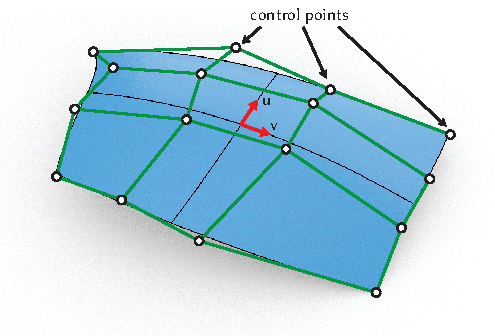
\includegraphics[width=\columnwidth]{figures/nurbs_patch}
    \caption{A cubic NURBS patch with 16 control points.}
    \label{fig:NURBS}
\end{figure}

The three-dimensional position, $\defX$, of any point on a NURBS surface can be written as 
\begin{equation}
\label{eqn:nurbs_srf}
\defX\left(u,v\right) = \sum_{i=1}^n\sum_{j=1}^n \phi_{ij}\left(u,v\right)\vc{q}_{ij},
    %\mathbf{x}(u,v) = \frac{\sum_{i=1}^{n}\sum_{j=1}^{m}  \mathbf{p}_{i,j} w_{i,j} B_{i,k}(u)B_{j,l}(v)}
    %{\sum_{i=1}^{n}\sum_{j=1}^{m} w_{i,j} B_{i,k}(u)B_{j,l}(v)}
    %\text{,}
\end{equation}
where $u$ and $v$ $\in \real$ are the coordinates of the 2D parametric domain, $n$ and $m$ are the number of control points in the $u$ and $v$ directions, $\mathbf{q}_{ij}\in\real^3$ are the control points and $\phi_{ij}\left(u,v\right)\in\real$ are the NURBS
basis functions given by 
\begin{equation*}
    \phi_{ij}\left(u,v\right) = \frac{w_{i,j}B_{ik}(u)B_{jl}(v)}{\sum_{r=1}^{n}\sum_{s=1}^{m} w_{ij} B_{ik}(u)B_{jl}(v)},
\end{equation*} where $B_{ik}$ (resp $B_{jl}$) is the $i^{th}$ ($j^{th}$) b-spline basis of order $k$ ($l$). 

Exploiting linearity with respect to the control points  we can express this mapping as 
\begin{equation}
    \defX\left(u,v\right) = \underbrace{\begin{pmatrix} \phi_{11}\left(u,v\right)\ident & \dots & \phi_{nn}\left(u,v\right)\ident \end{pmatrix}}_{\Jnurbs\left(u,v\right)}
    \underbrace{\begin{pmatrix} \vc{q}_{11} \\ \vdots \\ \vc{q}_{nn}\end{pmatrix}}_{\vc{q}},
\end{equation} where $\Jnurbs\left(u,v\right)$ is the NURBS Jacobian, $\ident$ is the $3\times3$ identity matrix and $\vc{q}$ is the vector of generalized coordinates~\dave{cite Lanczos}.
The Shape Matching Element Method will follow from this kinematic description.

\section{Shape Matching}
\label{sec:shapematching}

We begin by describing shape matching to a single NURBS part. 
Given a two different configurations of the same part (specified by the control points), shape matching computes a polynomial deformation which best aligns them.

Let $\vc{q^0}$ be the initial control points of the part, provided by the modeller and Let $\vc{q}$ be a vector of modified control point values.
We can compute the undeformed (or reference) position of any point on our part using $\refX\left(u,v\right) = \Jnurbs\left(u,v\right)\mathbf{q^0}$ and the corresponding
deformed (world space) position as $\defX\left(u,v\right) = \Jnurbs\left(u,v\right)\mathbf{q}$.

We can define a polynomial deformation from $\refX = \begin{pmatrix} X & Y & Z \end{pmatrix}^T$ to $\defX$  as 
\begin{equation}
    \defX\left(\refX\right) = 
    \underbrace{\begin{pmatrix}
    \mathbf{p}^T(\refX-\bar{\refX}) & \mathbf{0} & \mathbf{0} & 1 & 0 & 0\\
    \mathbf{0} & \mathbf{p}^T(\refX-\bar{\refX}) & \mathbf{0} & 0 & 1 & 0\\
    \mathbf{0} & \mathbf{0} & \mathbf{p}^T(\refX-\bar{\refX}) & 0 & 0 & 1\\
    \end{pmatrix}}_{\Pmatx}
    \Pcox,
    \label{eq:projection}
\end{equation} where $\mathbf{p}^T\left(\refX\right)$ is the polynomial basis vector \newline (eg $\begin{pmatrix} X & Y & X\cdot Y & X\cdot X & Y\cdot Y \end{pmatrix}$ ),
$\bar{\refX}$ is an a priori chosen origin around which to deform, $\Pco$ are the coefficients for the 
non-constant part of the polynomial and $\tr$ is the translation of the deformation origin. 
We can compute the shape matching deformation by solving~\cite{10.1145/1073204.1073216}
\begin{equation}
   \Pcox^* = \arg\min_{\Pco,\tr} \int \left\lvert\left\lvert\Pmatx\Pcox - \Jnurbs\vc{q}\right\rvert\right\rvert^2_2 dudv,
\end{equation} where we have suppressed the dependence of $\refX$ and $\Jnurbs$ on $u$ and $v$ for the sake of brevity.

\dave{Ty: need some text to explain how we pick points on the nurbs surface.}
\ty{Need to think a little more on how to write this. The main idea is that each surface has a knot vector and each Bspline covers a span of those knots. Therefore to guarantee we represent all control points for a surface, we uniformly sample $d+1$ points in each span, where $d$ is the NURBS surface}
We discretize the shape matching energy and minimize by solving
\begin{equation}
\samp{\Pmat}^T\wt\samp{\Pmat}\Pcox = \samp{\Pmat}^T\wt\samp{\Jnurbs}\vc{q}.
\label{eq:shapematch}
\end{equation} Here $\samp{\Pmat}$ (resp. $\samp{\Jnurbs}$) is a $3s \times 3k$ (resp. $3s \times 3nm$) matrix where $s$ is the number of quadrature points, 
$k$ is the number of  terms in the shape matching polynomial and $3nm$ is the number of NURBS control points. 
$\samp{\Pmat}$ (resp. $\samp{\Jnurbs}$) is constructed by stacking the evaluations of $\Pmatxuv$ (resp. $\Jnurbs\left(u, v\right)$) at each
quadrature point.
$\wt$ is a diagonal, $3s \times 3s$ matrix of integration weights.

\paragraph*{Relationship to the Virtual Element Method}
For a non-planar NURBS part, and given a sufficient number of quadrature points, ~\refeq{shapematch} will be well-posed allowing us to write: $\Pcox^* = \Pi\vc{q}$ where
\begin{equation*}
    \Pi = \left(\samp{\Pmat}^T\wt\samp{\Pmat}\right)^{-1}\samp{\Pmat}^T\wt\samp{\Jnurbs},
\end{equation*} is a projection from the space of control points onto the space of polynomials. 
This projection serves an identical purpose (and is mathematically equivalent up to choice of metric) to the projection operator used in VEM~\cite{10.1142/S021820251440003X}.
VEM uses a single polynomial projection per polyhedral element to solve differential equations on complex volumetric meshes.
We interpret shape matching as converting our NURBS part into a single Virtual Element suitable for elastodynamics simulation.
Unfortunately a single polynomial deformation space will not be suitably expressive for even moderately complex models. 
Previous work~\cite{10.1145/1073204.1073216,10.1145/1275808.1276480} used additional lattices or partitions of the reference space to 
increase the number of polynomials in the shape matching. Next we outline our meshless Shape Element Method which works directly on the NURBS
geometry itself.

\section{Shape Matching Element Method}
 Each input object is composed of a set of boundary representations, $\Prts$, one for each part $\prt\in\Prts$. 
 Our kinematic mapping is a blended construction (as is done for skinning~\cite{10.1145/2614028.2615427}) which we write as

 \begin{equation}
    \defX\left(\refX\right) = \sum_{\prt_i\in\Prts} \bld_i\Pmatxi\Pi_i\vc{q}_i, 
    \label{eq:kinematics}
 \end{equation} where $w_i$ $\Pmatx_i$, $\Pi_i$ and $\vc{q}_i$ are the blending weights, polynomial basis, projection operator and control points for the $i^{th}$
 part respectively.  
 
 \subsection*{Multiple Part Projection}
As in ~\refsec{shapematching} we construct each $\Pi_i$ via shape matching. 
It is tempting to use an identical polynomial basis matrix, $\Pmatx$ for all parts, $\prt_i$, but recall that constructing $\Pmatx$ requires the selection of a deformation
origin $\bar{\refX}$~(\refeq{projection}). 
Using the same origin for all polynomials limits the expressivity of the kinematic model~\cite{STBS:2011}.
Instead we choose a number of points in $\refX$ ($|\Prts| > |\XBs| > 0$, where $\XBs$ is the set of points)  to act as deformation origins~(\refsec{origins}).
For each part we now construct $\Pmatxi$ using the associated deformation origin $\bar{\refX}_j\in \XBs$, where each origin can
be shared between multiple parts.

\begin{figure}[h]
    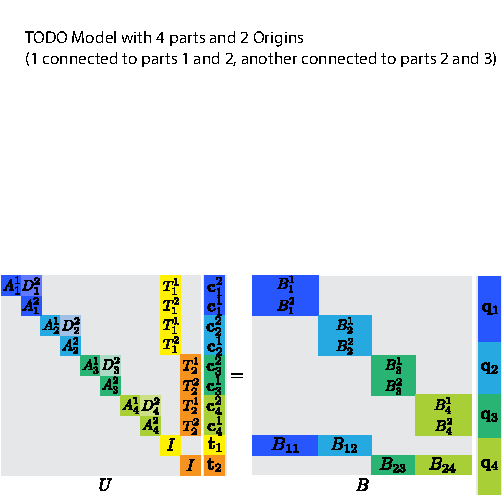
\includegraphics[width=\columnwidth]{figures/projection_operator_solve}
    \caption{A simple, four part model with two deformation origins and the corresponding matrix equation for the quadratic coefficients.}
    \label{fig:multiparts}
\end{figure}


Attempting to use $\Pmatxi$ in~\refeq{shapematch} on a per-part basis is problematic as it can become ill-posed, especially for planar boundary representations. 
To alleviate this problem we invoke the \emph{hierarchical ordering principle}, which argues that the behavior of a system is typically 
dominated by lower order effects~\cite{li2006regularities}. 
Mechanically, this principle suggests that the amount of motion modelled by increasingly high-order polynomials is decreasing. 
This implies that we can achieve acceptable shape matching results by performing shape matching hierarchically -- starting with the constant term and then 
fitting the remaining deformation with progressively higher-order deformations. 

For a given part, $\prt_i$, with associated origin $\bar{\refX}_j$ we first estimate the constant term, $\tr_i$ as the centroid of all parts associated with $\bar{X}_j$.
We next fit the linear part of the deformation by performing linear shape matching to $\prt_i$. 
This can be repeated for polynomials of arbitrary high order, for instance here we apply this approach to quadratic shape matching:
\ty{is the -1 above the A terms intentional? unsure if this is a common thing or an error}
\begin{equation}
    \begin{split}
        \tr_i  & = \sum_{\prt_k \in \bar{\refX}_j} \underbrace{\mathbbm{1}^T\wt_k \samp{\Jnurbs}_k}_{B_{ik}}\vc{q}_k \\
        \vc{c}_i^1 & = \underbrace{\left(\samp{\Pmat^1}^T\wt_i\samp{\Pmat^1}\right)}_{A^1_i}^{-1}\bigg(\underbrace{\samp{\Pmat^1}^T\wt_i\samp{\Jnurbs}_i}_{B^1_i}\vc{q}_i-\underbrace{\samp{\Pmat^1}^T\wt_i\mathbbm{1}}_{T^1_i}\tr_i\bigg)\\
        \vc{c}_i^2 & = \underbrace{\left(\samp{\Pmat^2}^T\wt_i\samp{\Pmat^2}\right)}_{A^2_i}^{-1}\bigg(\underbrace{\samp{\Pmat^2}^T\wt_i\samp{\Jnurbs}_i}_{B^2_i}\vc{q}_i-\underbrace{\samp{\Pmat^2}^T\wt_i\samp{\Pmat^1}}_{D^2_i}\vc{c}_i^1 - \underbrace{\samp{\Pmat^2}^T\wt_i\mathbbm{1}}_{T^2_i}\tr_i\bigg)
    \end{split},
    \label{eq:hfit} 
\end{equation} where $\Pmat^l$ contains only the monomial basis of order $l$,  $\samp{\Pmat^1}$ is the stacked evaluation of this matrix at $n$ quadrature points and $\vc{c}^l_i$ are the corresponding coefficients. 
Finally, $\wt_i$ is the diagonal integration weight matrix and $\mathbbm{1}\in\real^{3n\times3}$ is a matrix of stacked $3\times3$ identity matrices -- one for each quadrature point.


%%single projector for every object
When assembled for all parts,~\refeq{hfit}, yields a block upper triangular matrix $U$ and a spare matrix $B$ ~(\reffig{multiparts}) which can be used to efficiently to compute the projection 
operator for the entire object $\Pi = U^{-1}B\vc{q}$. 
The structure of $U$ and $B$ ensures that $\Pi$ only couples objects which share deformation centers, which implies a sparse $\Pi$. 
The per-part projection operators $\Pi_i$ correspond to blocks of rows of $\Pi$. 
Coupling via the deformation origins ensures our method will reproduce rigid and linear deformations in regions around these points, while higher order 
terms help compensate for more local deformations.

\dave{should have done Chebyshev shape matching to ensure higher order terms are orthogonal which would gaurantee exact reconstruction}

\subsection{Meshless Blending Weight Computation}
\label{sec:weights}
% \dave{Desireable Properties}
% \dave{Construction via post normalization}
% \dave{only need blending weights at quadrature points and surface samples so given sparse set of quadrature points compute blending weights using raycasting}
% \dave{things to explain (1) raycasting works for overlapping geometric, seperated geometry (2) weights glue objects together}
% \dave{maybe but weight figure here so reviewers immediately know that it looks pretty good}
% \dave{need to mention Monte Carlo Geometry processing but can't use it because our parts can overlap and that's a tricky boundary condition}

Our kinematic map~(\refeq{kinematics}) requires blending weights in order to homogenize our per-part representation. 
Specifying weights manually would be antithetical to our goal of providing a seamless translation from surface representation to physics-based animation.
Automatic  weight computation is a well-studied topic (see ~\citet{10.1145/2766952,BBW:2011} and ~\citet{10.1145/2010324.1964968}) but typically requires solving 
an optimization problem that itself relies on a volumetric discretization. 
This can be avoided by using stochastic methods~\cite{Sawhney:2020:MCG} but these do not yet support the boundary conditions we require for our problem. 

Ideally our shape functions would both partition unity and obey the Kronecker delta property (the $i^th$ blending function is one at $i^th$ part and zero on all other parts).
These properties ensure that our simulation can properly represent translation and that the solution stored at each part is the actual deformed position.
Additionally we would like our weights to be sparse both for performance reasons (leads to sparse matrices) and for expressivity (leads to locality of deformation). 

While partition of unity and sparsity are straightforward to enforce, the overlapping and intersecting parts~(\reffig{badmodels}) often encountered in non-engineering models leads
to a contradiction -- how can the blending functions be both one and zero at the points of overlap ? 
Our solution is to allow weights to include bounded discontinuities at these points and it is these discontinuous boundary conditions that are difficult to enforce 
with previous methods. 
\dave{ideally need a didactic figure showing this}

Given a set of reference space points $\st{X}$ inside our model, we want to evaluate $\bld_i\left(\refX_j\right)$, where $\bld_i$ is the weight function associated with 
the $i^{th}$ part, $\prt_i$, and $\refX_j\in\st{X}$. 

For each $\refX_j$ we find the nearest point on $\prt_i$, $\clst$.
We cast a ray from $\clst$, towards $\refX_j$ and find the intersection with the nearest part, $\rhit$.

\dave{Ty: How do we deal with non-planar parts ? What if the ray cast hits the same part that the closest point is on?}
\ty{Right now this doesn't happen as we only test intersection against other parts}

Next we compute two distances, $d_{\text{primary}}$, the distance from $\mathbf{X}_j$ to $\clst$ and $d_{\text{total}}$ the distance from  $\clst$ to $\rhit$.
Using these two distances we define a linear \emph{distance weight} using the well-known ReLU function:
\begin{equation}
\theta_i = \max (1.0 - \frac{d_{\text{primary}}}{\min (d_{\text{total}}, \alpha)}, 0.0)
\text{,}
\end{equation}
where $\alpha$ is a distance cutoff parameter. 
This distance weight~\reffig{plot_distance_weight} is the result of interpolating along this ray from $\clst$ to $\rhit$ (or a fixed point that depends on $\alpha$). 
These weights obey the Kronecker delta property for all parts but does not partition unity.

\begin{figure}[h]
    \centering
    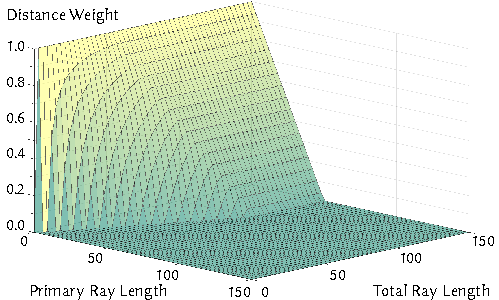
\includegraphics[width=3.33in]{figures/plot_distance_weight.pdf}
    \caption{We plot the distance weight with respect to the primary and total ray length. Here the cutoff distance is 50.
    }
    \label{fig:plot_distance_weight}
    \vspace{-5pt}
  \end{figure} 

%\begin{figure}
%    \includegraphics[width=\columnwidth]{example-image-a}
%    \caption{Figure showing how weight calculation works (left) ray casting plus result (right) after correcting for partition of unity}
%    \label{fig:weightcompute}
%\end{figure}

Next we use these distance weights to compute our final blending weights.
At each $\refX_j$ we want to compute $\mathbf{\bld}(\mathbf{X}_j) =  \left( \bld_1(\mathbf{X}_j), \dots, \bld_n(\mathbf{X}_j) \right)$, where 
$\sum_{i=1}^n\bld_i(\mathbf{X}_j) = 1$, and each $\bld_i \geq 0$, which we enforce by solving a local optimization problem: 

\begin{equation}
\begin{aligned}
\mathbf{w}(\mathbf{X}_j) =  \arg\min_{\mathbf{w}} \quad & \mathbf{w}^T \Theta(\mathbf{X}_j) \mathbf{w}    \\
\textrm{st} \quad & 0 \leq w_i \leq 1 \mbox{ }\forall i                    \\
                  &   \sum_i^n w_i = 1                      \\
\end{aligned}
\end{equation}

where $\Theta(\mathbf{X}) = \text{diag}\left( \frac{1}{\theta_1},\frac{1}{\theta_2},\dots,\frac{1}{\theta_n}\right)$. 

This post-process ensures that our blending weights partition unity and are non-negative~(\reffig{distance_weight_puft}). 
For any point on a part that is non-intersecting, the weights will satisfy the Kronecker delta property since the inverse distance weights imply that only
a single theta will have a non-infinite weight. 
For points that lie on more than one part, the weights associated with the intersecting parts will be equal and all others will be zero
In other words, the deformed positions of these intersecting points will be an average, which is a plausible solution and ensures continuity.
The blending weights immediately jump back to one and zero for non-intersecting points on each part. 
Finally, the distance cutoff $\alpha$ allows us to control the sparsity of the blending weights.

\begin{figure}[h]
    \centering
    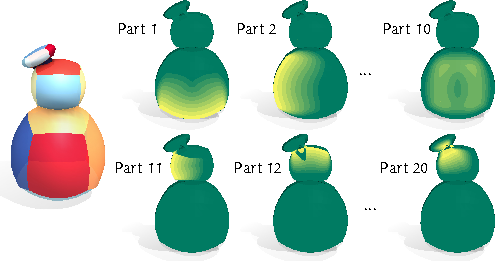
\includegraphics[width=3.33in]{figures/distance_weight_puft.pdf}
    \caption{Our blending weights decay smoothly from 1.0 (yellow) to 0.0 (green) when moving away from its closest surface. Here we visualize the distribution of the distance weights (with cutoff distance 5.0) corresponding to each part.   
    }
    \label{fig:distance_weight_puft}
    \vspace{-5pt}
  \end{figure} 
  %
  %

Using raycasting to compute blending weights imbues our method with similar advantages to \citet{Sawhney:2020:MCG} (allowing us to 
handle intersecting geometry, geometry with gaps and to perform constructive solid geometry operations on the fly),
but allows us to use more general weighting functions and apply the appropriate behavior for intersecting parts.
The price we pay for these advantages is that our weights are not C0 continuous but rather Lipchitz smooth.
Perturbations in the boundaries of parts can cause bounded jumps in our distance weights. 
However these jumps occupy an infinitesimal percentage of the volume of our object are easy to avoid when integrating
physical quantities, leaving our simulation unaffected. 

\subsection{Choosing Deformation Centers}
\label{sec:origins}
\dave{Ty: try to follow this formula when writing 
\dave{maybe this should come after weight computation ?}
(1) what is the purpose of this part of the method ?
(2) what are the criteria for success
(3) what is our assumed input 
(4) what is the desired output
(5) what's the algorith,
(6) add proofs/diagrams/figures that show we satisfy (2). }
To ensure kinematic expressiveness, it is essential that multiple origins of deformation are permitted. Each part, $\prt_i$, must be associated with a single deformation origin, $\bar{\refX}_j$. Each origin is computed as the centroid of the set of parts with which it is associated. While we constrain a part to be paired with only one deformation origin, an origin may be associated any number of parts. Next, we require that each deformation origin be associated with a minimum of two parts, which avoids the case of an origin laying on the surface of a part.\ty{Should we mention periodic surfaces? You can have a periodic nurbs sphere consisting of a single surface, which we couldn't handle with this constraint (easy fix, but not sure if worth mentioning)} Furthermore, we seek that the sparsity of the deformation origins mirrors that of the blending weights. Intuitively, this means that for a region in which weights are high for a subset of parts, the origin of deformation should be centered in this region.

\begin{figure}[h]
    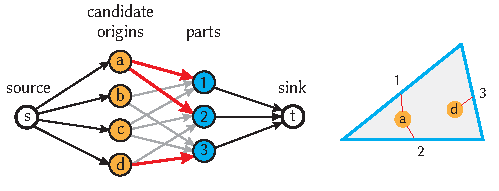
\includegraphics[width=\columnwidth]{figures/origin_network}
    \caption{Example structure for the network flow selection of deformation origins with a shape consisting of three parts. Red arrows indicate each parts origin association.}
    \label{fig:network_flow}
\end{figure}

From the set of blending weights we seek to construct a set of candidate deformation origins and then produce a set of deformation origins, $\XBs$, adhering to the outlined requirements. This set of candidate origins is identified by examining the unique combinations of weight assignments for the quadrature points. For each $\refX_j$, we form a set $\mathbf{c}\left(\refX_j\right)$ with $c_i\left(\refX_j\right)= 1-\delta_{\bld_i\left(\refX_j\right),0}$ where $\delta_{x,0}$ is the Kronecker delta. This produces a binary code for each quadrature point that identifies the parts to which this point has nonzero weights. We use each unique binary code as a deformation origin candidate.

With the set of requirements and candidate origins, we see this problem may be organized in a graph structure ~(\reffig{network_flow}) where the relationships between parts and deformation origins can be realized as a bipartite graph. We exploit this structure by forming a min-cost-flow problem that produces a solution satisfying the requirements.

Consider a directed bipartite graph $G=(V = A \cup B,E)$ where each node in $A$ corresponds to a deformation origin candidate and each node in $B$ represents a part. $E$ is the set of edges connecting nodes in $A$ to $B$ where each origin has an edge to every part with which it attempts to associate. We augment $G$ to form $G'=(V' = A \cup B \cup \{s,t\}, E')$ where $V'$  is the new set of nodes now containing the source, $s$, and sink, $t$, nodes. $E'$ is the augmented set of nodes connecting $s$ to each candidate in $A$ and connecting each part in $B$ to the sink $t$. Each edge $(i,j) \in E'$ has an associated flow $f_{ij}$ and capacity constraint $u_{ij}$, and each edge in $E'$ also has a cost $c_{ij}$. The principal constraint for this network flow problem is the conservation constraint, meaning that the net flow for all nodes in $V$ is zero.

First, we constrain all flow values to be integral and place a capacity of $1$ on the edges from $B$ to $t$. This has the effect of enforcing that any part node in $B$ receives flow from a single edge, and as a consequence each part may only be associated with a single deformation origin.  With the specified network and constraints, we solve this problem with an integer constrained linear program. We choose $\XBs$ to be all nodes in $A$ that have an outgoing flow of at least $1$.


\subsection{Meshless Integration}

We integrate physical quantities over our undeformed object using raycasting based quadrature~\cite{KHOSRAVIFARD201030}.

\dave{Ty: a bit more here, show the transformation of the integral via divergence theorem then show the final discrete version. Clearly define the quadrature rules.}

We make a minor modifiction this procedure to handle common geometric pathologies encountered in NURBS modeling, such as overlapping surfaces by performing 
CSG unions while raycasting\dave{find a citation}. 
The output of this raycasting procedure is a set of quadrature points $\st{X}$ and weights $\st{v}$ that we use for integration and also as input to our 
deformation origin extraction~\refsec{origins} and blending weights computation~\refsec{weights}
\reffig{raycasting} shows the convergence of this quadrature approach when used to compute the volume of a NURBS model.
\begin{figure}
    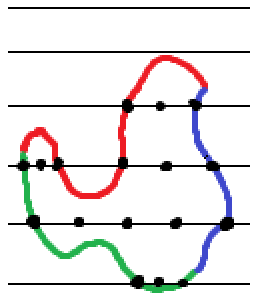
\includegraphics[width=\columnwidth]{figures/raycasting_quadrature}
    \caption{Figure showing how raycasting quadrature works (top), convergence plot for volume integration (bottom}
    \label{fig:raycasting}
\end{figure}

\section{Physics-Based Animation}


\subsection{Mass Matrix}
The kinetic energy for a model may be expressed as
\begin{equation}
T = \frac{1}{2}\int_{ \Omega} \rho \dot{\mathbf{x}}^T\dot{\mathbf{x}} d\Omega
\text{,}
\end{equation}
where $\Omega$ is the 3D integration domain, $\rho$ is the density, and $\dot{\mathbf{x}}$ is the velocity for some point in the domain. Using the deformation map defined in \ref{eqn:compact_x_map}, we may rewrite this kinetic energy as
\begin{equation}
\begin{split}
T & = \frac{1}{2}\int_{ \Omega} \rho \dot{\mathbf{q}}^T \mathbf{J}^T\mathbf{Y(X)}^T\mathbf{Y(X)}\ d\Omega \\
  & = \frac{1}{2} \dot{\mathbf{q}}^T \mathbf{J}^T \left[ \int_{ \Omega} \rho \mathbf{Y(X)}^T\mathbf{Y(X)} d\Omega \right] \mathbf{J}\dot{\mathbf{q}} \\
  & = \frac{1}{2} \dot{\mathbf{q}}^T \mathbf{M} \dot{\mathbf{q}}
\end{split}
\text{.}
\end{equation}
The second line is a result of the fact that all terms except for $\mathbf{Y(X)}$ are spatially constant, allowing us to move these outside the volume integral, which enables fast assembly of the mass matrix, $\mathbf{M}$.

\subsection{Error Energy}
\dave{We should cite VEM literature and point out this is a standard thing they do to make the algorithm consistent and convergent}
Over the course of the simulation we may see the true boundary values deviate from their positions estimated by the polynomial. This is most notable in cases where the degree of the polynomial on a NURBS is higher than the degree of the B-spline surface. To address this we augment our kinetic energy with a term to account for this error. The error for a boundary point $\mathbf{x}_i^*$ that is known to lie on the limit surface of the NURBS can be written as
\begin{equation}
\begin{split}
\epsilon_i & = ||\mathbf{x}(\mathbf{X}_i) - \mathbf{x}_i^*|| \\
		   & = ||(\mathbf{Y}(\mathbf{X}_i)\mathbf{L} - \mathbf{S_i})\mathbf{\hat{b}}||
\end{split}
\text{,}
\end{equation}
where $\mathbf{S_i}$ extracts $\mathbf{x}_i^*$ from $\mathbf{\hat{b}}$. We modify this error further to be expressed in terms of the control points. We note that $\mathbf{x}^*(u,v)$ yields the position on the NURBS surface whereas $\mathbf{x(X)}$ is the deformed value estimated by the polynomial fitting. Furthermore $\mathbf{X}$ may be written as a function of the parametric coordinates $\mathbf{X}(u,v)$ as its position on the surface is produced using the initial set of control points representing the undeformed model. This leads to an energy potential over the NURBS surface in parametric space
\begin{equation}
T_E = \iint (\mathbf{x}(\mathbf{X}(u,v)) - \mathbf{x}^*(u,v))^T(\mathbf{x}(\mathbf{X}(u,v)) - \mathbf{x}^*(u,v)) du dv
\text{.}
\end{equation}
The discrete form of this written in terms of the control points may be written as
\begin{equation}
\begin{split}
T_E & = \sum_i^N  \dot{\mathbf{q}}^T\mathbf{J}^T(\mathbf{Y}(\mathbf{X}_i)\mathbf{L} - \mathbf{S_i})^T(\mathbf{Y}(\mathbf{X}_i)\mathbf{L} - \mathbf{S_i})\mathbf{J}\dot{\mathbf{q}} \\
  & = \dot{\mathbf{q}}^T\mathbf{J}^T \left[ \sum_i^N  (\mathbf{Y}(\mathbf{X}_i)\mathbf{L} - \mathbf{S_i})^T(\mathbf{Y}(\mathbf{X}_i)\mathbf{L} - \mathbf{S_i}) \right] \mathbf{J}\dot{\mathbf{q}} \\
  & = \dot{\mathbf{q}}^T \mathbf{M}_E \dot{\mathbf{q}}
\end{split}
\text{,}
\end{equation}
where $N$ is the total number of boundary points and $\mathbf{M}_E$ is our \textit{error mass matrix}.
% \subsection{Generalized Forces}
% We write our potential energy as 
% \begin{equation}
%     V = \int_\Omega \psi(\mathbf{F(X)}) d\Omega
% \text{.}
% \end{equation}
% To evaluate this energy (as well as its derivatives), we require a definition for the deformation gradient, $\mathbf{F(X)}$:
% \begin{equation}
%         \mathbf{F(X)} = \frac{\partial \mathbf{x}}{\partial \mathbf{X}}
%                = \frac{\partial \mathbf{Y(X)}}{\partial \mathbf{X}}\mathbf{L}\hat{\mathbf{b}}
% \text{.}
% \end{equation}
% In the expression for the deformed position $\mathbf{x(X)}$ we see that the dependence on $\mathbf{X}$ only exists in $\mathbf{Y(X)}$, making $\mathbf{L}$ and $\hat{\mathbf{b}}$ constant terms when compute $\mathbf{F}$. Full details on how to compute $\mathbf{F}$ and its derivative $\frac{\partial \mathbf{F}}{\partial \mathbf{q}}$ may be found in the appendix. (\myworries{I just wrote this because I'm too tired to right the d etails right now :p}. Now that we have an expression for the deformation gradient, we discretize our potential energy as follows
% \begin{equation}
%     V =  \sum_i^m \psi(\mathbf{F(X}_i) A_i
% \text{,}
% \end{equation}
% where $m$ is the number of integration points and $A_i$ is the volume for the $i$-th integration point.

% Like in the case of the kinetic energy, we also introduce an error force potential, which takes the simple form
% \begin{equation}
% V_E = \mathbf{q}^T \mathbf{M}_E \mathbf{q}
% \end{equation}
\subsection{Deformation Gradient}
\dave{gotta deal with this weight gradient}
At this point we have shown how to fit a polynomial describing the deformation of each surface. With these polynomial coefficients coupled with their associated centers of mass, we can construct an estimate of some arbitrary material point $\mathbf{X}$ using the deformation described by the surface. This lends itself to a general definition for the deformed position of a point as a weighted sum of the polynomials, which yields a unique polynomial for the point. Thus we arrive at a definition for the deformed position, $\mathbf{x}$, of a material point $\mathbf{X}$ in the undeformed space:
\begin{equation}
\label{eqn:deformation_map}
	\mathbf{x}(\mathbf{X}) = \sum_i^n w_i(\mathbf{X}) \left[ \mathbf{M}(\mathbf{X-\bar{X}}_j)\mathbf{c}_i + \mathbf{t}_j \right]
	\text{,}
\end{equation}
where we have $n$ surfaces, and $w_i$ and $\mathbf{c}_i$ are the weights and the coefficients for the $i$-th surface, respectively. The terms $\mathbf{\bar{X}}_j$ and $\mathbf{t}_j$ the undeformed and deformed centers of mass, respectively, that are associated with the $i$-th surface.


\subsection{External Forces}
\dave{Jacobian transpose}

\subsection{Time Integration}
With our definition of the deformation map as well as a strategy for integrating the volume, we now have the necessary ingredient to perform dynamic simulation. We follow the Variational Mechanics approach that defines a pair of kinetic and potential energies, and we apply the Euler-Lagrange equation to develop our equations of motion.

Before we define these energies we first would like to simplify the form of the deformation map presented in equation \ref{eqn:deformation_map}. We may write $\mathbf{x}(\mathbf{X})$ in matrix form as
\begin{equation}
\mathbf{x}(\mathbf{X}) = \underbrace{\left[w_1\mathbf{M}(\mathbf{X - \bar{X}}_j) \dots w_n\mathbf{M}(\mathbf{X - \bar{X}}_j) \middle| \sum_i^{n_1}w_1^i\mathbf{I} \dots \sum_i^{n_m}w_m^i\mathbf{I} \right]}_{\mathbf{Y}(\mathbf{X})}
\begin{bmatrix}
\mathbf{\hat{c}} \\
\mathbf{\hat{t}}
\end{bmatrix}
\text{,}
\end{equation}
\myworries{I'm not sure how to write this matrix form for x(X), especially on finding the best notation for the center of mass indexing. So this above equation is temporary.}
where we have $n$ shape elements, $m$ centers of mass. We simplify the above equation and use the following form
\begin{equation}
\label{eqn:x_simple_form}
\mathbf{x}(\mathbf{X}) = \mathbf{Y}(\mathbf{X})\mathbf{L}\hat{\mathbf{b}}
\text{,}
\end{equation}
where we make use of equation \ref{eqn:c_multiple_elements} to rewrite this in terms of the boundary points $\mathbf{\hat{b}}$. As one final step, we rewrite this again in terms of the control points of our NURBS surfaces:
\begin{equation}
\label{eqn:compact_x_map}
\mathbf{x}(\mathbf{X}) = \mathbf{Y}(\mathbf{X})\mathbf{LJq}
\text{,}
\end{equation}
where we use the fact that $\mathbf{\hat{b}} = \mathbf{Jq}$. \myworries{not a fan of this, perhaps we change $\hat{b}$ to something else...} This gives us an expression for the deformed position in terms of our generalized coordinates, $\mathbf{q}$.

\dave{discrete Equations of motion with quadratured integrals, reference/details on how we handle collisions}

We have now provided all the necessary ingredient to produce equations of motion for deformable bodies, which we derive via Euler-Lagrange equation. We begin with the Lagrangian
\begin{equation}
    L=(T+T_E)-(V + V_E)
\end{equation}
Then from the Euler-Lagrange equation we have:
\begin{equation}
    \frac{d}{dt} \frac{\partial L}{\partial \dot{\mathbf{p}}} + \frac{\partial L}{\partial {\mathbf{p}}} = 0
\end{equation}
\myworries{todo: not totally sure what to write here since we're experimenting with both linearly implicit backward euler as well as Newton's method soon}



\begin{equation}
   \frac{\partial L}{\partial \mathbf{q}} = \sum_i^m \frac{\partial V_i}{\partial \mathbf{q}} = \sum_i^m \frac{\partial \psi(\mathbf{F_i)}}{\partial \mathbf{F}}\frac{\partial \mathbf{F_i}}{\partial \mathbf{q}}A_i
\end{equation}
\

\dave{Some extra notes on how we handle collisions, add a reference, just say we do this from here.}
%%% ------- OLD STUFF BELOW --------
% \section{Methods}
% \dave{We should probably put some pseudo code for the preprocessing and the runtime algorithms right up fron, along with a quick textual walk through of the method.}
% Given a volumetric model composed of one or more NURBS surfaces, the surface of each surface is reconstructed using a set of control points $\textbf{p}$ and their associated weights $w$. Following D-NURBS \cite{10.1145/176579.176580}, we take our degrees of freedom (DOF) to be control points of the surfaces and produce displacements directly on these control points at each simulation step. We note that we used a simplified version of D-NURBS in which the weights are held constant throughout the simulation and find this not to be limiting \myworries{(feel like we'll need better justification than saying just this?)}. We represent the degrees of freedom for the $i$-th NURBS surface with $m$ control points as $\mathbf{q}_i = \left[ \mathbf{p}_1^T, \dots, \mathbf{p}_m^T \right]^T \in \mathbb{R}^{3m}$. From this definition, we write the DOF for the entire model as $\mathbf{q} = \left[ \mathbf{q}_i^T, \dots, \mathbf{q}_n^T \right]^T$ where $n$ is the number of NURBS surfaces for the model. 

% To evaluate the volumetric integrals in solid mechanics models, we require material points $\mathbf{X} \in \mathbb{R}^{3m}$ in the undeformed space that serve as integration points. Our shape matching element method enables us to evaluate the deformed positions of the material points strictly using positions defined on the boundary. Like in VEM, we fit a polynomial to each boundary primitive (NURBS in this case) describing its deformation. The fitting of these polynomials closely follows that of the Shape Matching \cite{10.1145/1073204.1073216} approach where we perform a least squares polynomial fit to the deformed boundary points. These boundary points are represented by sampled positions on each NURBS surface. Since each surface is associated with a single polynomial, we can construct a unique polynomial for some arbitrary point by blending these polynomials. Thus given some material point $\mathbf{X}_i$ we find it's corresponding deformed position $\mathbf{x}_i$ via a weighted combination of the polynomials. This permits us to build a general deformation map which we use to construct our equations of motion.

% In the following sections, we will first review the simplified D-NURBS model used to form our generalized coordinates. We then present our shape matching algorithm for fitting polynomials to surfaces .... In section ... we next describe how to blend these surface polynomials to construct a general deformation map for material points. Section ... describes our strategy for selecting integration points in the volume through a raycasting approach. Finally, we formulate our equations of motions from a Lagrangian formulation.

% \section{D-NURBS Model}
% \myworries{TODO: Most of these matrices should be paranthesis matrices}
% We provide a brief overview of the D-NURBS formulation presented in \cite{10.1145/176579.176580}. Our models in our method are composed of a collection of NURBS surfaces. 

% \subsection{D-NURBS Formulation}
% A point on a NURBS surface is typically expressed in the following form
% \begin{equation}
% \label{eqn:nurbs_srf}
%     \mathbf{x}(u,v) = \frac{\sum_{i=1}^{n}\sum_{j=1}^{m}  \mathbf{p}_{i,j} w_{i,j} B_{i,k}(u)B_{j,l}(v)}
%     {\sum_{i=1}^{n}\sum_{j=1}^{m} w_{i,j} B_{i,k}(u)B_{j,l}(v)}
%     \text{,}
% \end{equation}
% where where have a total of $nm$ control points $\mathbf{p}$ and weights $w$. Using the B-spline basis functions and the weighted control points, this formula gives a map from our parametric coordinates $u,v$ to their corresponding position on the surface in $\mathbb{R}^{3m}$. $B_{i,k}(u)$ is the B-spline basis function for the $i-th$ control point with degree $k-1$.

% We would like our generalized coordinates to be the control points of the model so that the dynamics operates directly on the original representation. Therefore, we would like to rewrite equation \ref{eqn:nurbs_srf} in the form
% \begin{equation}
%     \mathbf{x}(u,v) = \mathbf{J}(u,v)\mathbf{q}
%     \text{,}
% \end{equation}
% where $\mathbf{q} = \left[ \mathbf{p}_{1,1}^T, \dots, \mathbf{p}_{i,j}^T, \dots, \mathbf{p}_{n,m}^T \right]^T \in \mathbb{R}^{3nm}$ is the set of $nm$ control points \myworries{in the overview I just write $n$ control points, but here i'm writing $nm$} for a single NURBS surface arranged as a column vector. $\mathbf{J} \in  \mathbb{R}^{3 x 3nm}$ is the NURBS jacobian that maps $(u,v)$ coordinates to world positions in $\mathbb{R}^{3}$.

% The NURBS jacobian, $\mathbf{J}$, is a matrix composed of horizontally concatenated $3x3$ blocks where the $(i,j)$-th block is $\frac{\partial \mathbf{x}}{\partial \mathbf{p}_{i,j}}$ for the $(i,j)$-th control point. $\frac{\partial \mathbf{x}}{\partial \mathbf{p}_{i,j}}$ is a diagonal $3x3$ matrix where each diagonal entry $N_{i,j}(\mathbf{u})$ takes the form

% \begin{equation}
% \label{eqn:jacobian_diagonal}
%     N_{i,j}(u,v)
%     = \frac{w_{i,j} B_{i,k}(u)B_{j,l}(v)}{\sum_{i=1}^{n}\sum_{j=1}^{m} w_{i,j} B_{i,k}(u)B_{j,l}(v)}
%     \text{.}
% \end{equation}
% Thus the NURBS jacobian for a single $(u,v)$ pair is written as
% \begin{equation}
% \label{eqn:uv_jacobian}
%     \mathbf{J}(u,v) =
%     \left[ \frac{\partial \mathbf{x}}{\partial \mathbf{p}_{1,1}} \dots
%            \frac{\partial \mathbf{x}}{\partial \mathbf{p}_{i,j}} \dots 
%            \frac{\partial \mathbf{x}}{\partial \mathbf{p}_{n,m}}
%     \right]
%     \text{.}
% \end{equation}

% This formulation is a simplification of the full D-NURBS described in \cite{10.1145/176579.176580} the weights of the NURBS are fixed throughout the simulation. Permitting the dynamics to modify weights would likely improve the expressiveness of the kinematics, but we find fixing the weights affords sufficiently expressive results and improves performance. The performance improvement is a result of having fixed $N_{i,j}(u,v)$ entries over the course of the simulation. The full D-NURBS model requires rebuilding the jacobian and consequently the mass matrices at each time step. 

% \subsection{Generalized Coordinates for a NURBS model}
% The above formulation describes developing the map from a single $(u,v)$ coordinate to its corresponding position on the surface. In our simulation we represent the entire boundary of the NURBS model, so we require samples along each surface. We emphasize that we only require an initial selection of $(u,v)$ coordinates across each surface and the dynamics of the simulation modifies the set of control points $\mathbf{q}$ to modify the world space maps $\mathbf{x}(u,v)=\mathbf{J}(u,v)\mathbf{q}$.

% Let's say for a NURBS surface on the model the DOF column vector is $\mathbf{q}_i$, which is the subset of control points in the generalized coordinates for the $i$-th surface. For a given surface with $m$ pairs of $\mathbf{u}=(u,v)$ coordinates sampled in parametric space, we write the jacobian for the $i$-th surface as \myworries{(should I use something like $\hat{\mathbf{J}}$ instead?)}
% \begin{equation}
% \label{eqn:surface_jacobian}
%     \mathbf{J}_i =
%     \left[ \mathbf{J}(\mathbf{u})_1^T \dots \mathbf{J}(\mathbf{u})_m^T \right]^T
%     \text{.}
% \end{equation}
% Then if $\mathbf{x}_i$ is the set of $m$ world space positions for the $i$-th surface, we may write $\mathbf{x}_i = \mathbf{J}_i \mathbf{q}_i$. Finally, given the full set of generalized coordinates $\mathbf{q} = \left[ \mathbf{q}_i^T, \dots, \mathbf{q}_n^T \right]^T$ with $n$ surfaces, we may write jacobian $\mathbf{J}$ for the entire model as a block diagonal matrix:
% \begin{equation}
% \mathbf{J} = \left[ \begin{array}{ccccc}
% \mathbf{J}_1 &  &  &  &  \\
%  & \ddots &  &  &  \\
%  &  & \mathbf{J}_i & &  \\
%  &  &  & \ddots &  \\
%  &  &  &  & \mathbf{J}_n \\
% \end{array} \right]
% \text{.}
% \end{equation}
% With this equation, the full set of world positions of the NURBS model may be written as $\mathbf{x} = \mathbf{J}\mathbf{q} \in \mathbb{R}^{3N}$ where $N$ is the total number of $(u,v)$ coordinates.


% \subsection{Shape Matching with Multiple Elements}

% \subsection{Computing the Blending Weights}


% \subsection{Generalized Inertia}



% \subsection{Time Integration}
% 

%
\section{Results and Discussion}

\begin{table*}[h]
  \caption{Performance of, and parameters for the Shape Matching Element Method on all examples. All timings are reported in seconds, physical  parameters are
  reported with appropriate units. $\rho$ is the applied density, \textbf{E} is the  Young's Modulus and $\mu$ is the Poisson's ratio.
  }
  \label{tbl:perf}
  \begin{center}
  \begin{tabular}{l c c c c c c c c c c}
   \textbf{Example} $|\vc{q}|$ & \textbf{Material}&  $\rho$(kg/m$^3$) & \textbf{E}(GPa) & $\mu$ &\textbf{Sample Model}(s) & \textbf{Quadrature}(s)& \textbf{Weights}(s)& \textbf{Build $\Pi$}(s)& \textbf{Step}(s)\\
   \hline 
   \rowcolor[HTML]{DAE8FC} 
   \textbf{Cantilever}      & ? & ? & ? & ? & ? & ? & ? & ? & ? & ? \\
   \textbf{Coffee mug}      & ?& ? & ? & ? & ? & ? & ? & ? & ? & ?  \\
   \textbf{Rocket}          & ?& ? & 648 & ? & ? & ? & ? & ? & ? & ?\\
   \textbf{Castle}          & ?& ? & ? & ? & ? & ? & ? & ? & ? & ?\\
   \textbf{Chicken}        & ? & ? & ? & ? & ? & ? & ? & ? & ? & ?\\
   \textbf{Starship}       & ? & ? & ? & ? & ? & ? & ? & ? & ? & ?\\
   \textbf{Tire}           & ? & ? & ? & ? & ? & ? & ? & ? & ? & ?\\
   \hline
  \end{tabular}
  \end{center}
  
  \end{table*}

%\dave{we should show the nurbs model in rhino/fusion for every example, maybe an exploded view as well}

%\dave{mention that not so many standard NURBS models so we modelled lots of these ourselves .. show's power of approach that we can model and sim all these examples.}

%\dave{use as many different meshes as possible for figures (i.e try not to have the same mesh show up in more than one figure if possible).}

%\dave{we should report which models we made ourselves}
We implemented SEM in a combination of MATLAB and C++ using both GPToolbox~\cite{gptoolbox} and Bartels~\cite{bartels} for geometry processing and constitutive models 
respectively. Benchmarks were performed using a  ~\dave{CPU} with \dave{xx}MB of RAM.

\reftbl{perf} shows the size of all our examples along with performance statistics and relevant parameters.
Note that the individual parts of all models are \emph{not connected}, and no continuity constraints or constructive solid geometry operations have been applied. 
Rather, the SEM approach implicitly couples the boundary parts together to allow for seamless volumetric simulation. 
Models were created using Autodesk Fusion 360 \cite{AutodeskFusion360} and Rhinocerous 3D 7 \cite{mcneel-rhinoceros}.
  
For raycasting operations and rendering we rely on Embree~\cite{10.1145/2601097.2601199} and triangulate the NURBS surfaces, which only represents an implementation simplification. 
Our algorithm is not dependent on triangulating the boundary, and an ideal alternative would be using a path tracer.

\nicetohave{Would be nice to mention TNURBS, which would give us a good reason to include the wrench (which i really wanna do). I doubt we have time to do a 3 point bending test, but a simple elastic wrench simulation would be easy to cook up}
For handling trimmed NURBS surfaces, we augment our sampling of the surfaces by using raycasting integration in 2D. Trimmed NURBS may be defined by a boundary curve in the parametric space, so we raycast to find intersection intervals in the UV space on which quadrature points are generated. For rendering Trimmed NURBS, we discretize the the boundary curve as a polyline and use triangle \cite{shewchuk96b, SHEWCHUK200221} to form a boundary conforming triangulation. The vertices of this triangulation serve as fixed set of high resolution UV samples for constructing a render mesh.


%% Results that relate to preprocessing
% weights are good
% \begin{figure}
%   \centering
%   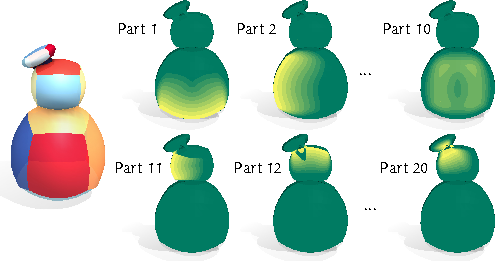
\includegraphics[width=3.33in]{figures/distance_weight_puft.pdf}
%   \caption{Our distance weights decay smoothly from 1.0 (yellow) to 0.0 (green) when moving away from its closest surface. Here we visualize the distribution of the distance weights (with cutoff distance 5.0) corresponding to each part.   
%   }
%   \label{fig:distance_weight_puft}
%   \vspace{-5pt}
% \end{figure} 
% %
% %
% \begin{figure}
%   \centering
%   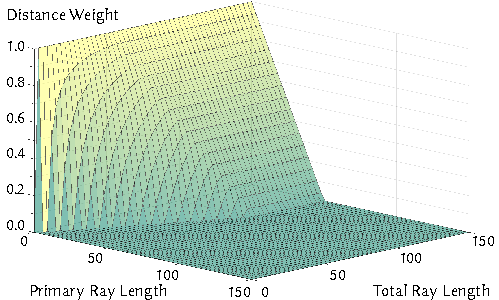
\includegraphics[width=3.33in]{figures/plot_distance_weight.pdf}
%   \caption{We plot the distance weight with respect to the primary and total ray length. Here the cutoff distance is 50.
%   }
%   \label{fig:plot_distance_weight}
%   \vspace{-5pt}
% \end{figure} 

%kinematic model is expressive
% \begin{figure}
%   \includegraphics[width=\columnwidth]{example-image-a}
%   \caption{Take an intesting geometry (maybe that geometry processing cacture), deform it, do our shape matching and then reconstruct the deformed pose. Do this for a bunch of poses (show's kinematic model is good).}
%   \label{fig:deform}
% \end{figure}

%% Results that relate to simulation output
%correctness
\begin{figure}[h]
  \includegraphics[width=\columnwidth]{figures/patch_test.pdf}
  \caption{2D patch test. By applying affine transformations to the boundary of the original undeformed model (left), we show that solving the static problem gives rigid motion for rotation and constant strain for shearing and stretching (right).}
  % \caption{2D patch test. Left: the original undeformed model defined by four surface elements on the boundary. Right:  applying affine transformations to the boundary and show that solving the static problem gives rigid motion for rotation and constant strain for shearing and stretching}
  \label{fig:patchtest}
\end{figure}


We first validate the physical plausibility of our method using a small 2D patch test~(\reffig{patchtest}). 
Here the test object is a square made of four edges (not joined at the corners) simulated using linear polynomials with a single deformation center.
We apply a battery of boundary conditions and resolve the deformation of the element by minimizing the elastic potential.
We note that SEM is able to represent rigid motions, as well as shearing and anisotropic stretching. 
This implies that, with sparse weights, SEM can resolve these motions locally, leading to physically plausible simulation results.

We further demonstrate \emph{qualitative} convergence of SEM with respect to linear tetrahedral finite elements when increasing the number of patches in use.
In \reffig{convergence}, we compare identical cantilevered beams, simulated using a Neohookean constitutive model (Young's Modulus $=$ $0.001$ GPa, Poisson's Ratio $=$ $0.45$) and implicit time integration with a timestep of $0.01$s. 
We use SEM with quadratic polynomials for this test and observe that our SEM simulation, made of 24 independent NURBS patches, shows good agreement with FEM. Each subdivision of the NURBS beam enables more complicated kinematics, 
but very few surface elements are needed to produce compelling results.

\begin{figure}[h]
  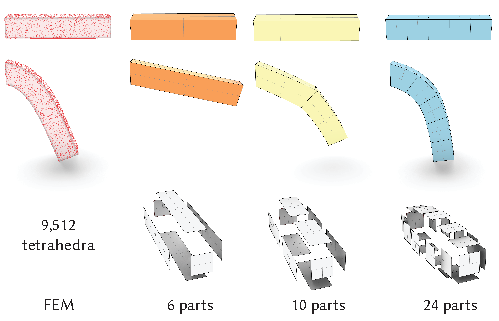
\includegraphics[width=\columnwidth]{figures/beams.pdf}
  \caption{Our SEM simulation is able to qualitatively converge to a high resolution FEM simulation result (left) as we increase the number of surfaces in the model (right). }
  \label{fig:convergence}
\end{figure}

We also show that our raycasting weight computation is able to create shape-aware output. \reffig{independence} shows that manipulating
parts that are nearby but separated will behave in an appropriately independent fashion. Our grumpy model is capable of extending 
its leg without causing unrealistic deformations in the plant foot.

\begin{figure}[h]
  \includegraphics[width=\columnwidth]{figures/independent_movement}
  \caption{Our raycasting weight computation produces share-aware blending weights. Here the locality of our blending weights allows the two legs of the grumpy model to move independently. }
  \label{fig:independence}
\end{figure}

% relaxed modelling constraints
By virtue of its meshless nature, SEM is robust to a wide range of challenging models with large gaps and disconnected primitives.
\reffig{fig:chicken} shows frames from a simulation of a rubber chicken. Note that the chicken model itself features large gaps between the individual NURBS parts. 
Despite the lack of explicit connectivity, the SEM blending weights have the effect of implicitly enforcing connectivity at these seams. 

\begin{figure*}[htp]
  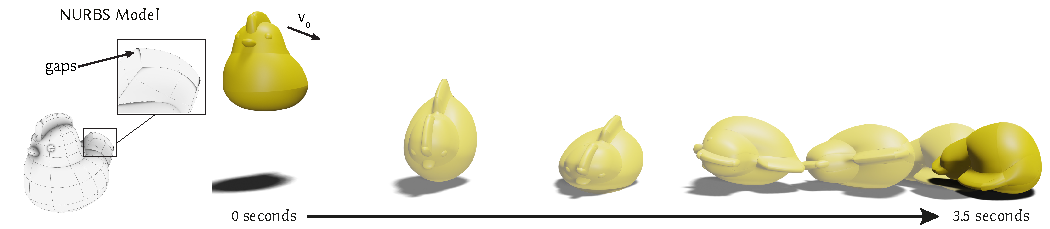
\includegraphics[width=\textwidth]{figures/chicken.pdf}
  \caption{Simulation of a chicken model with gaps between surfaces.}
  \label{fig:chicken}
\end{figure*}

SEM is also robust to intersections in modelling input. \reffig{badmodels} shows simulations of two jelly coffee mugs. 
The top row shows a model with negligible overlap, whereas the bottom row shows the result of a careless modeller who has deeply embedded the handle of the mug in the body in order to attach it, creating a large area of overlap.
In both cases SEM produces a plausible physically-based animation without requiring additional model clean-up.

\begin{figure}[H]
  \includegraphics[width=\columnwidth]{figures/mug_overlap}
  \caption{Our SEM is robust to overlapping regions and self-intersections. Here the simulation result of the coffee mug with overlapping handle (bottom) still matches its corresponding counterpart without negligible overlaps (top). }
  % \caption{Coffee mug with overlapping handle. (top) row of models with increasing overlap (middle) single weight image showing behaviour in the overlapping region, (bottom) simulation result for each one}
  \label{fig:badmodels}
\end{figure}

%different material parameters / material models 
Since the equations of motion for SEM are derived using a general elastic potential, it is theoretically capable of supporting arbitrary elastic constitutive models.
% We derive the equations of motion for SEM using a general elastic potential and thus SEM supports arbitrary constitutive models. 
\reffig{rocket} shows a rocket ship simulated with both high stiffness (steel) and low stiffness materials (rubber). 
In both cases intuitive and visually pleasing results are created wherein the trajectories correctly reflect the desired material characteristics.  
%multiple materials
\begin{figure*}[htp]
  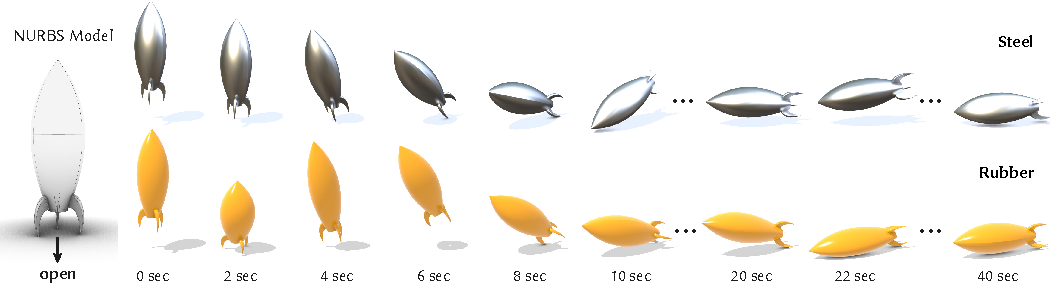
\includegraphics[width=\textwidth]{figures/rocket.pdf}
  \caption{SEM is able to produce animation using a wide variety of material parameters. Here we simulate both a steel and rubber rocket ship. 
  To make this even more challenging, the rocket model is an open surface (at the bottom), but a plausible animation is still generated.}
  \label{fig:rocket}
\end{figure*}

SEM also supports the simulation of objects made up of heterogenous materials. By specifying different material properties inside nested 
parts we are able to simulate a drag racing wheel with a metal hub and soft rubber tread~(\reffig{tire}).

\begin{figure}[h]
  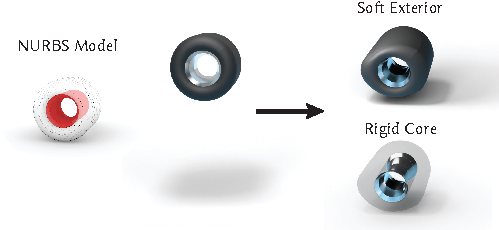
\includegraphics[width=\columnwidth]{figures/tire}
  \caption{Our SEM is directly applicable to the simulation of objects with heterogenous materials.}
  \label{fig:tire}
\end{figure}


% %different surface reps
% Though we focus on NURBS surface representations, the only NURBS specific construction in the SEM method is the Jacobian \refeq{velocity_jacobian}.
% Many other boundary representations admit a linear representation and are thus directly consumable by our method.
% \reffig{subd} shows an example of applying our SEM method to a subdivision model by making such a modification.
% \begin{figure}[h]
%   \includegraphics[width=\columnwidth]{example-image-a}
%   \caption{show subd simulation if we have it. If it works really well we'll just mix subds and nurbs throughout the paper. }
%   \label{fig:subd}
% \end{figure}

% different time integration scheme
\nicetohave{Integration Figure}
%\begin{figure}[h]
%  \includegraphics[width=\columnwidth]{example-image-a}
%  \caption{show mug simulation using newton's method, linearly implicit Euler \Honglin{Maybe I can do that quickly}. }
%  \label{fig:time_integration}
%\end{figure}

%editing example
For downstream applications, the output of  SEM simulation is itself editable in a NURBS modelling program (see \reffig{edit}). 
This can be useful for visual effects pipelines, allowing artists to easily post process animations using the same tools in which they were created.
\begin{figure}[h]
  \includegraphics[width=\columnwidth]{example-image-a}
  \caption{Here we show the output of an SEM animation loaded into Rhinoceros 3D 7 for additional editing.}
  \label{fig:edit}
\end{figure}

%show stoppers
Finally we show a few additional examples, highlighting the ability of SEM to handle complex simulations involving deformation, contact and friction.
In \reffig{staypuft} we show two astronauts in jaunty space suits collide in zero gravity while in \reffig{starship} 
we show an animation of the Space-V starship landing on Mars in a graceful way.

\begin{figure*}[htp]
  \includegraphics[width=\textwidth,height=3in]{example-image-a}
  \caption{Two astronauts, in jaunty spacesuits collide while spacewalking in zero-g.}
  \label{fig:staypuft}
\end{figure*}

\begin{figure*}[htp]
  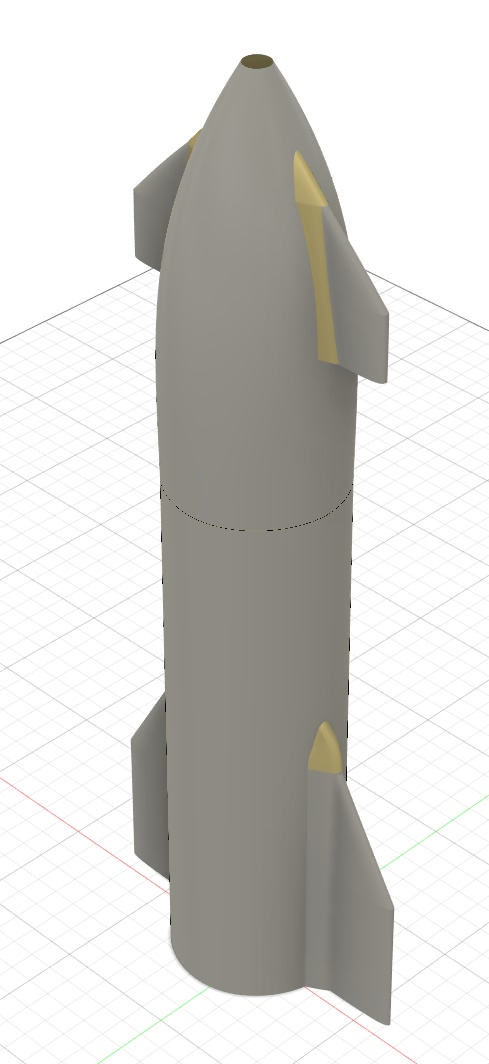
\includegraphics[width=\textwidth,height=3in]{figures/starship.pdf}
  \caption{The Space-V starship makes a graceful landing on the red planet. }
  \label{fig:starship}
\end{figure*}

\section{Future Work and Conclusions}
\dave{mention that constraint from complimentary dynamics could be used to replace error energy}
We have presented the Shape Matching Element Method (SEM), the first completely meshless approach to direct simulation of NURBS models.
Our approach is unique in its ability to infer volumetric shape from surface only models,
including ones with intersecting geometry, between parts and other defects common to non-engineering models.
Our method allows simulation of such input directly, with a variety of contitutive models and time integration schemes
and is compatibale with standard methods for collision resolution. 
We believe that SEM is a signficant improvement over standard physics-based animtion pipelines for NURBS models. 
As evidence of the efficacy of our approach, the authors submit that many of the examples in this paper were constructed ourselves
(since the standard graphics menagerie is not available as NURBS models). 
Modelling, cleaning, meshing and simulating would've been a burdensome experience without SEM's
ability to leap directly from (often hastily) constructed models to physics-based animations.

But SEM as it's presented here is only the beginning and we believe there are many exciting areas of future work to explore.
We are very excited to couple SEM to machine learning approaches for design, parameter estimation and Real2Sim applications.
One of the cumbersome elements in using finite element simulation for such problems is the need for robust, differentiable volumetric meshing.
While there has been some work on this~\dave{cite} it is far from a solved problem.
SEM removes this bottleneck entirely, providing a direct mapping from geometric input to physics-driven output. 
We believe this will both enable simpler and more robust algorithms for  physics-based ML and 
allow the application of such algorithms to a much broader class of problems. 

SEM itself has much room for addition.
First, while we focus on NURBS surfaces here, the only part of SEM that is NURBS specific is the shape matching operation.
We believe there is potential to allow mixed models (models which include polygonal meshes, particles, subdivision surfaces and NURBS)
by extending the range of shape matching operations used by the algorithm. The shape matching operation itself could be improved to be material aware 
(to better handle heterogenous materials) or to be robust to noisy data (allowing direct simulation of scanned data). The Finite Element method took over 
40 years to take over the world of simulation. 
We see this work as the first step in a similar journey for SEM

To encourage future research on SEM the authors will release our SEM implementation under a permissive license as well as all models created for this submission.


%%
%% The next two lines define the bibliography style to be used, and
%% the bibliography file.
\bibliographystyle{ACM-Reference-Format}
\bibliography{references}

\end{document}
